\section{Selection Sort} \label{cap:2:section:ssort}

\subsection{Introdução}

O Selection Sort é um algoritmo de ordenação relativamente eficiente com número de entradas baixo,
seu funcionamento consiste em consumir o vetor a ser ordenado de forma sequencial buscando pelo menor
elemento do vetor e inserindo-o na posição correta.

\subsection{Implementação}

Para o algoritmo de ordenação baseado em seleção, o pseudo-código utilizado para desenvolver o
algoritmo pode ser observado em \ref{selectionSortP}.

\begin{pseudocode}[caption={Algoritmo de ordenação por seleção}, label={selectionSortP}]
SELECTION-SORT(A)
n $\gets$ len(A)
i $\gets$ 1
while i < n - 1 do
    min $\gets$ i
    j $\gets$ i + 1
    while j < n do
        if A[j] < A[min] then
            min $\gets$ j
    if i $\neq$ min then
        swap(A[i], A[min])
    i $\gets$ i + 1
\end{pseudocode}

Esse pseudo-código foi implementado na linguagem de programação C 
e pode ser observado no código seguinte:

\begin{lstlisting}[style=CStyle]
void sSort(int * v, int n)
{
    int min;
    for (int i = 0; i < n - 1; i++)
    {
        min = i;
        for (int j = i + 1; j < n; j++)
        {
            if (v[j] < v[min])
            {
                min = j;
            }
        }
        if (i != min)
        {
            swap(&v[i], &v[min]);
        }
    }
}
\end{lstlisting}

\subsection{Análise do algoritmo e notação assintótica}

Para que seja determinada a razão de crescimento do algoritmo de ordenação por seleção, é necessário
perceber os tempos de execução de cada linha do pseudo-código \ref{selectionSortP}.
Nesse caso, pode-se ter como base a equação \ref{cap:2:eq:selectionSort:1}.

\begin{equation} \label{cap:2:eq:selectionSort:1}
    T(n) = C_2 + C_3 + \sum_{i=1}^{n - 1}(C_4 + C_5 + C_6 + C_9 + C_{10} + C_{11} + C_{12}) + \sum_{j=1}^{n^2}(C_7 + C_8) 
\end{equation}

Portanto, é plausível relacionar a equação \ref{cap:2:eq:selectionSort:1} com a equação \ref{cap:2:eq:selectionSort:2}.

\begin{equation} \label{cap:2:eq:selectionSort:2}
    T(n) = an^2 + bn + c \  para\  a = (C_7 + C_8),\  b = (C_4 + C_5 + C_6 + C_9 + C_{10} + C_{11} + C_{12})\  e\  c = (C_2 + C_3)
\end{equation}

Com isso, pode-se determinar as seguintes notações assintóticas para o algoritmo de ordenação 
por seleção:

\begin{align*} \label{cap:2:eq:selectionSort:3}
    O(n) &= n^x \forall x \geq 2 \\ 
    \Omega(n) &= n^x \forall x \leq 2 \\
    \Theta(n) &= n^2
\end{align*}

\subsection{Comparação teórica-prática}

Para melhor compreensão do tempo de execução do algoritmo de ordenação por seleção, pode-se observar o gráfico 
\ref{cap:2:graph:selectionSort} que apresentam o tempo de execução para o algoritmo de ordenação por seleção
para 2048 casos diferentes com o número de entradas $n$ variando de 1 a 65536.

\begin{figure}[h]
    \centering
    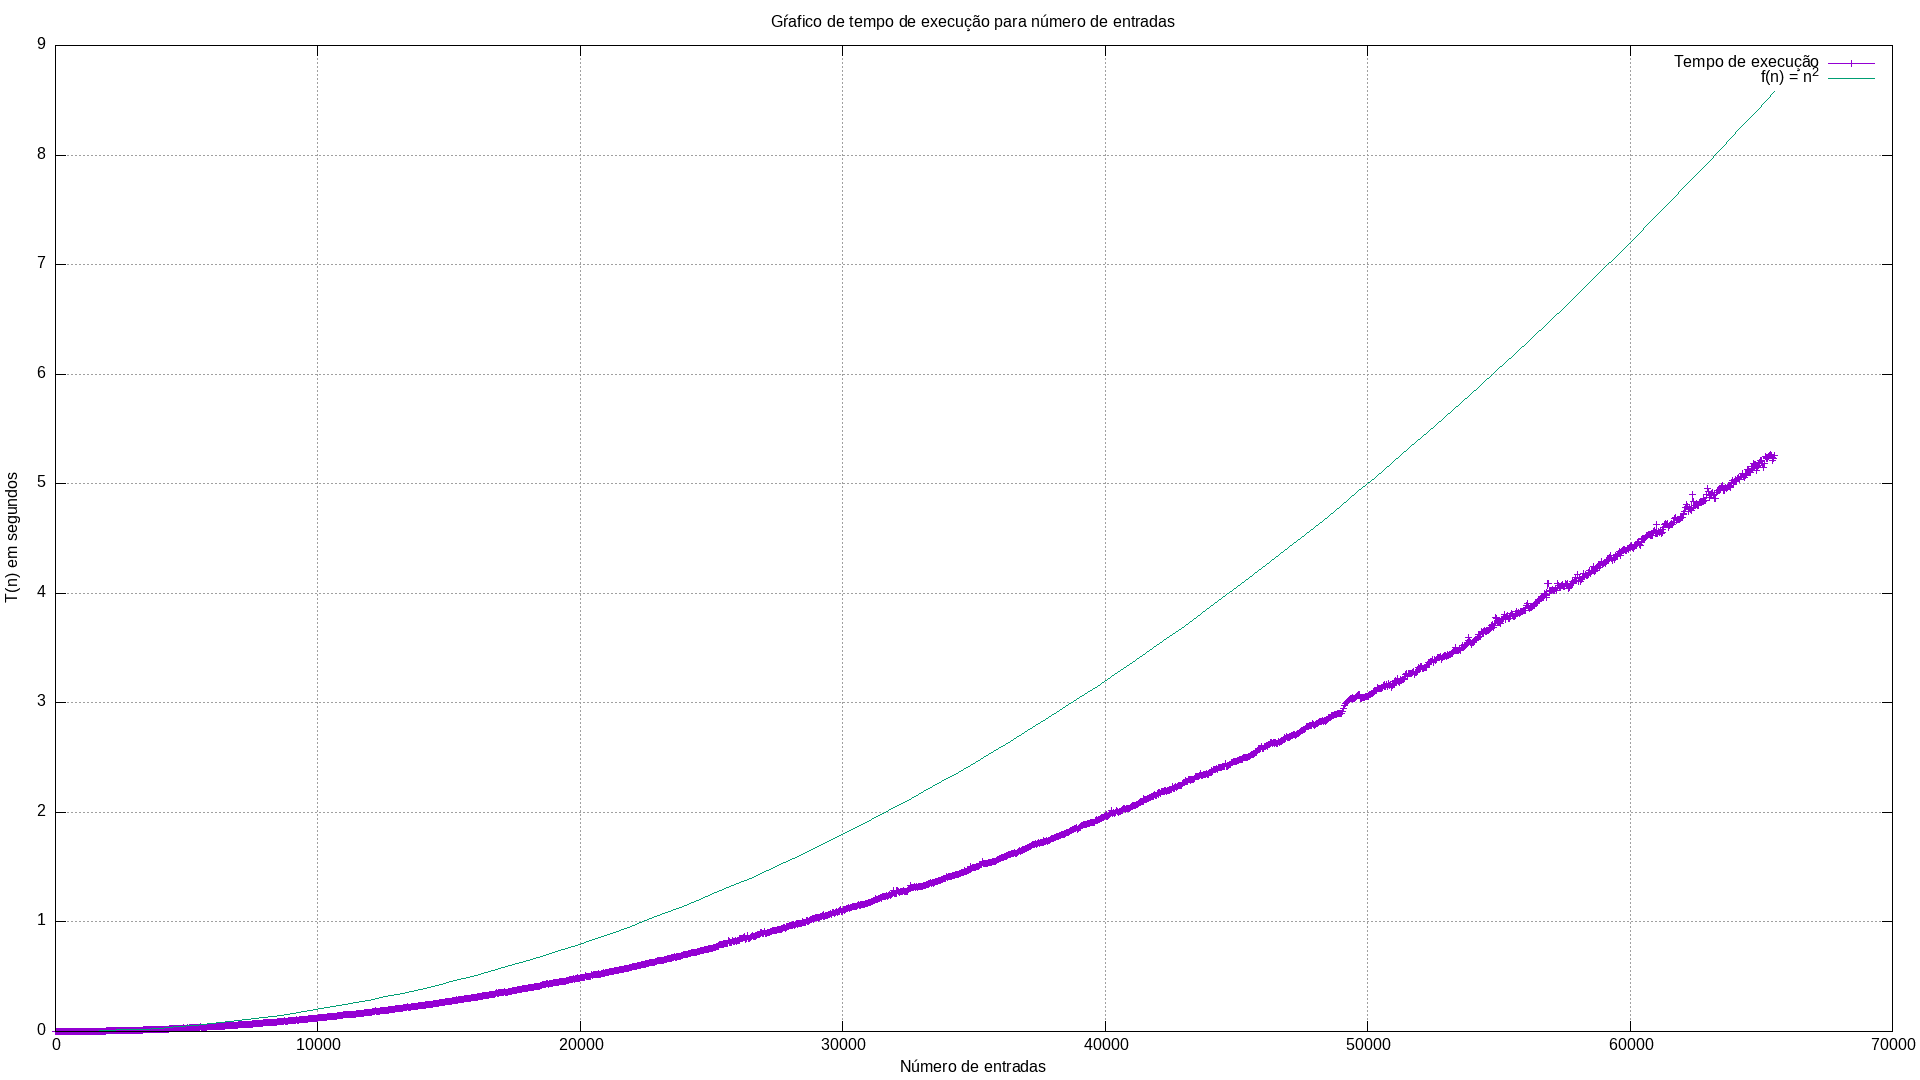
\includegraphics[width=\textwidth]{image/graphics/selectionSort.png}
    \caption{Gráfico com tempo de execução do algoritmo de ordenação por seleção}
    \label{cap:2:graph:selectionSort}
\end{figure}

No gráfico \ref{cap:2:graph:selectionSort}, é possível perceber que o tempo de execução do algoritmo se aproxima
da função $f(n)$ que é uma função quadrática para $n$ com uma redução de escala para melhor percepção e comparação. Então,
utilizando como base o gráfico \ref{cap:2:graph:selectionSort}, pode-se confirmar que a ordem de crescimento determinada é
precisa.

\subsection{Discussão sobre tempo de execução e uso de memória}

Sobre seu tempo de execução, o algoritmo de ordenação por seleção é eficiente para vetores
com poucas entradas a partir de um certo limiar e do contexto, existem outros algoritmos de ordenação
mais eficientes que o mesmo. Sobre seu uso de memória, é constante porque utiliza apenas algumas variáveis
auxiliares.

